
% ----------------------------------------------------------------------
%  Set the document class
% ----------------------------------------------------------------------
\documentclass[11pt,a4paper,twoside]{article}

% ----------------------------------------------------------------------
% Define external packages, language, margins, fonts and new commands
% ----------------------------------------------------------------------
%\input{preamble} 
%\usepackage[utf8]{inputenc}   % <<<<< Linux
\usepackage[english]{babel} % <<<<< English
\usepackage{notoccite}
\usepackage[skip=0.5\baselineskip]{caption}
\usepackage[mathletters]{ucs}
\usepackage[utf8x]{inputenc}

\usepackage{mathtools}

\usepackage{listings}

%\usepackage[ascii]{inputenc}
\usepackage{siunitx}
\usepackage{lmodern}
\usepackage[T1]{fontenc}
\usepackage[babel=true]{microtype}




\makeatletter
\newread\pin@file
\newcounter{pinlineno}
\newcommand\pin@accu{}
\newcommand\pin@ext{pintmp}
% inputs #3, selecting only lines #1 to #2 (inclusive)
\newcommand*\partialinput [3] {%
  \IfFileExists{#3}{%
    \openin\pin@file #3
    % skip lines 1 to #1 (exclusive)
    \setcounter{pinlineno}{1}
    \@whilenum\value{pinlineno}<#1 \do{%
      \read\pin@file to\pin@line
      \stepcounter{pinlineno}%
    }
    % prepare reading lines #1 to #2 inclusive
    \addtocounter{pinlineno}{-1}
    \let\pin@accu\empty
    \begingroup
    \endlinechar\newlinechar
    \@whilenum\value{pinlineno}<#2 \do{%
      % use safe catcodes provided by e-TeX's \readline
      \readline\pin@file to\pin@line
      \expandafter\expandafter\expandafter\def\expandafter\expandafter\expandafter\pin@accu\expandafter\expandafter\expandafter{\expandafter\pin@accu\pin@line}
      %\edef\pin@accu{\pin@accu\pin@line}%
      \stepcounter{pinlineno}%
    }
    \closein\pin@file
    \expandafter\endgroup
    \scantokens\expandafter{\pin@accu}%
  }{%
    \errmessage{File `#3' doesn't exist!}%
  }%
}
\makeatother





\usepackage[all]{nowidow}
\usepackage[skip=2pt]{caption}
\usepackage{indentfirst}
\usepackage[dvipsnames]{xcolor}
\usepackage{verbatim}



\newcommand{\squeezeup}{\vspace{-4.5mm}}
%blind text
\usepackage{lipsum}

\usepackage{graphicx}
\graphicspath{ {./} {../../figlib/} }
\def\FontLn{% 16 pt normal
  \usefont{T1}{phv}{m}{n}\fontsize{16pt}{16pt}\selectfont}
\def\FontLb{% 16 pt bold
  \usefont{T1}{phv}{b}{n}\fontsize{16pt}{16pt}\selectfont}
\def\FontMn{% 14 pt normal
  \usefont{T1}{phv}{m}{n}\fontsize{14pt}{14pt}\selectfont}
\def\FontMb{% 14 pt bold
  \usefont{T1}{phv}{b}{n}\fontsize{14pt}{14pt}\selectfont}
\def\FontSn{% 12 pt normal
  \usefont{T1}{phv}{m}{n}\fontsize{12pt}{12pt}\selectfont}

% Use Arial font as default
\renewcommand{\rmdefault}{phv}
\renewcommand{\sfdefault}{phv}
\usepackage{geometry}	
\geometry{verbose,tmargin=2.5cm,bmargin=2.5cm,lmargin=2.5cm,rmargin=2.5cm}

%\usepackage{setspace}
%\renewcommand{\baselinestretch}{1.5}

\usepackage[pdftex]{hyperref} % enhance documents that are to be
                              % output as HTML and PDF
\hypersetup{colorlinks,       % color text of links and anchors,
                              % eliminates borders around links
%            linkcolor=red,    % color for normal internal links
            linkcolor=black,  % color for normal internal links
            anchorcolor=black,% color for anchor text
%            citecolor=green,  % color for bibliographical citations
            citecolor=black,  % color for bibliographical citations
%            filecolor=magenta,% color for URLs which open local files
            filecolor=black,  % color for URLs which open local files
%            menucolor=red,    % color for Acrobat menu items
            menucolor=black,  % color for Acrobat menu items
%            pagecolor=red,    % color for links to other pages
            %pagecolor=black,  % color for links to other pages
%            urlcolor=cyan,    % color for linked URLs
            urlcolor=black,   % color for linked URLs
	          bookmarks=true,         % create PDF bookmarks
	          bookmarksopen=false,    % don't expand bookmarks
	          bookmarksnumbered=true, % number bookmarks
	          pdftitle={report},
            pdfauthor={Andre C. Marta},
%            pdfsubject={Thesis Title},
%            pdfkeywords={Thesis Keywords},
            pdfstartview=FitV,
            pdfdisplaydoctitle=true}

\usepackage[numbers,sort&compress]{natbib} % <<<<< References in numbered list [1],[2],...
\usepackage{subcaption} 
\usepackage{mdframed}

%%%%%%%%%%%%%%%%%%%%%%%%%%%%%%%%%%%%%%%%%%%%%%%%%%%%%%%%%%%%%%%%%%%%%%%%
%     Begin Document                                                   %
%%%%%%%%%%%%%%%%%%%%%%%%%%%%%%%%%%%%%%%%%%%%%%%%%%%%%%%%%%%%%%%%%%%%%%%%


\begin{document}

% Set plain page style (no headers, footer with centered page number)
\pagestyle{plain}

% Set roman numbering (i,ii,...) before the start of chapters
%\pagenumbering{roman}

% ----------------------------------------------------------------------
%  Cover page
% ----------------------------------------------------------------------
%%%%%%%%%%%%%%%%%%%%%%%%%%%%%%%%%%%%%%%%%%%%%%%%%%%%%%%%%%%%%%%%%%%%%%%%
%                                                                      %
%     File: Thesis_FrontCover.tex                                      %
%     Tex Master: Thesis.tex                                           %
%                                                                      %
%     Author: Andre C. Marta                                           %
%     Last modified :  2 Jul 2015                                      %
%                                                                      %
%%%%%%%%%%%%%%%%%%%%%%%%%%%%%%%%%%%%%%%%%%%%%%%%%%%%%%%%%%%%%%%%%%%%%%%%

\thispagestyle {empty}

% IST Logo - Signature A
% parameters: bb=llx lly urx ury (bounding box), width=h_length, height=v_length, angle=angle, scale=factor, clip=true/false, draft=true/false. 
\includegraphics[bb=9.5cm 11cm 0cm 0cm,scale=0.29]{IST_A_CMYK_POS}

\begin{center}
%
% Figure (Image or plot)
\vspace{1.0cm}
% height = 50 mm
%\includegraphics[height=50mm]{Figures/Airbus_A350.jpg}

% Title, author and degree
\vspace{1cm}
{\FontLb Laboratory Report 3: AC/DC Converter} \\ % <<<<< EDIT TITLE
\vspace{1cm}
{\FontSn Circuit Theory and Electronics Fundamentals} \\
\vspace{1cm}
{\FontSn Department of Electrical and Computer Engineering, Técnico, University of Lisbon} \\ % <<<<< EDIT COURSE
\vspace{1cm}
{\FontSn April 8, 2021} \\ % <<<<< EDIT DATE (corresponds to date of oral examination)
\vspace{1cm}
{\FontSn Work by:} \\ 
\vspace{0.5cm}
{\FontSn Beatriz Contente 95772} \\ 
\vspace{0.5cm}
{\FontSn Francisco Fonseca 95789} \\ 
\vspace{0.5cm}
{\FontSn Manuel Carvalho 95823} \\ 
%
\end{center}


% ----------------------------------------------------------------------
% Dedication page (optional)
% ----------------------------------------------------------------------
%\input{dedication} 
%\cleardoublepage

% ----------------------------------------------------------------------
%  Acknowledgments (optional)
% ----------------------------------------------------------------------
%\input{acknowledgements}
%\cleardoublepage

% ----------------------------------------------------------------------
%  Abstract (both in English and Portuguese)
% ----------------------------------------------------------------------
%\input{resumo} 
%\cleardoublepage

%\input{abstract} 

% ----------------------------------------------------------------------
%  Table of contents, list of tables, list of figures and nomenclature
% ----------------------------------------------------------------------

% Table of contents
%
\tableofcontents

% List of tables
%\addcontentsline{toc}{section}{\listtablename}
%\listoftables
%\cleardoublepage 

% List of figures
%\addcontentsline{toc}{section}{\listfigurename}
%\listoffigures
%\cleardoublepage 

% Set arabic numbering (1,2,...) after preface
%
%\setcounter{page}{1}
%\pagenumbering{arabic}

% ----------------------------------------------------------------------
%  Body
% ----------------------------------------------------------------------

\section{Introduction}
\label{sec:introduction}

% state the learning objective 
The objective of this laboratory assignment is to do analysis on a circuit using the mesh and the nodal method as well as running a simulation using NGspice with the objective of detecting small diferences between the different studies and understand why said differences happens. The circuit can be seen in Figure~\ref{fig:rc}.

In Section~\ref{sec:analysis}, a theoretical analysis of the circuit is
presented. In Section~\ref{sec:simulation}, the circuit is analysed by
simulation, and the results are compared to the theoretical results obtained in
Section~\ref{sec:analysis}. The conclusions of this study are outlined in
Section~\ref{sec:conclusion}.

\begin{figure}[h] \centering
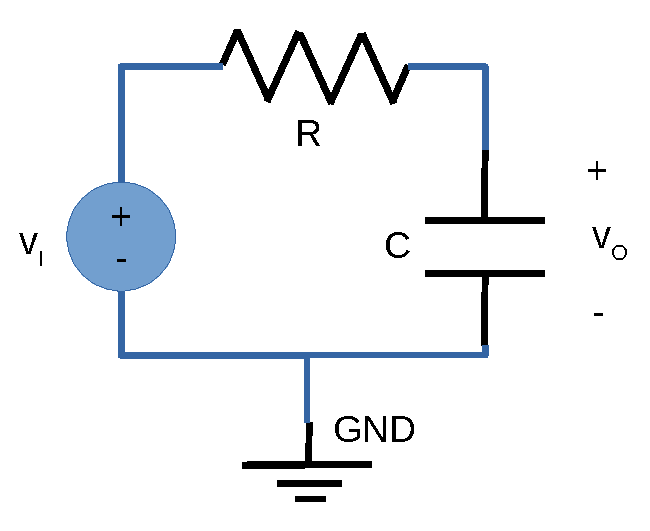
\includegraphics[width=0.5\linewidth]{rc.pdf}
\caption{Circuit with an independent current and voltage source ($V_a$ and $I_d$ respectively) and linear dependent sources ($V_c$-linear current controlled voltage source and $I_b$-linear voltage controlled current source}
\label{fig:rc}
\end{figure}



\newpage
\section{Theoretical Analysis}
\label{sec:analysis}

In this section we will present the answers to questions~\ref{sec:exercise1} to~\ref{sec:exercise6}. For solving purposes, all the unkown currents used in the node analysis were considered to be diverging from the node. The node $V_4$ is connected to the ground (GND) in every exercise, the voltage in it being 0V.

\label{sec:Exercise 1}
\begin{figure}[!ht] \centering
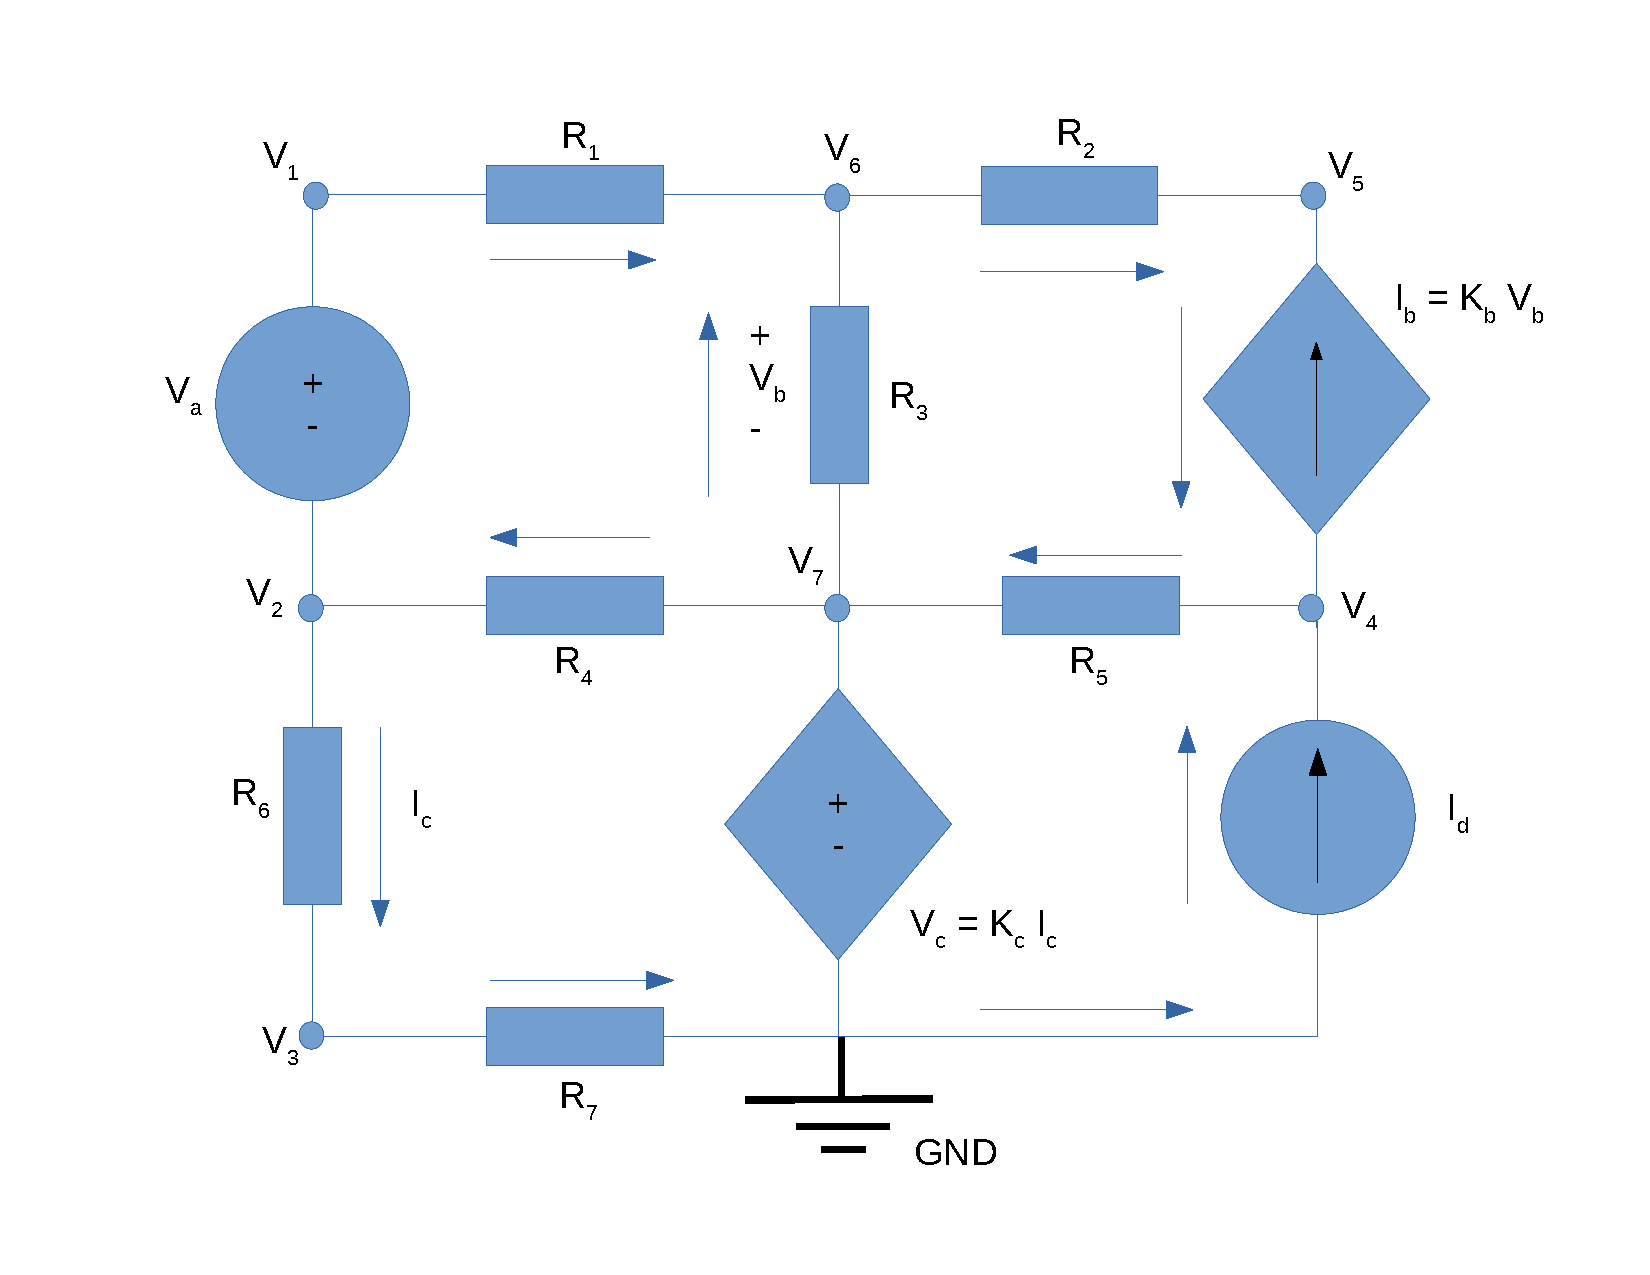
\includegraphics[width=0.8\linewidth]{circuit_final.pdf}
\squeezeup 
\caption{Representation of the current directions considered.}
\label{fig:theoretical}
\end{figure}

\subsection{Exercise 1}
\label{sec:exercise1}


%---------------Theoretical Analysis Exercise 1--------------------------------------------------------%
 
The first thing which must be noticed is that there is an independent voltage source ($V_s$) and a linear current controlled voltage source ($V_d$) in this circuit. Knowing that a nodal analysis can't include the analysis of nodes that are connected to voltage sources, it becomes clear that is useless to analyze nodes 1 and 4 (connected to $V_s$) and also nodes 5 and 8 (connected to $V_d$) using this method.

From figure~\ref{fig:theoretical}, we can easily conclude that there are 11 unknown variables: $V_b$, $I_b$, $V_d$, $I_d$, $V_1$, $V_2$, $V_3$, $V_5$, $V_6$, $V_7$ and $V_8$. In this exercise, $V_s$ is constant and the capacitor is assumed to be also constant and fully charged, meaning that the current $I_c$ is 0 (open circuit behavior).

For the node analysis, it is necessary to consider 7 linearly independent equations to reach all the values corresponding to the voltages in each node and consequently solve the circuit. As referred above, it is possible to use the nodal method to analyze nodes 2, 3, 6 and 7.

We begin by establishing the following equations, being that equations ~\ref{eq:given11} and ~\ref{eq:given12} were given by the professor. Equation ~\ref{eq:vb1} was obtained by relating the voltage difference between nodes 2 and 5 to the voltage $V_b$. Finally, by using Ohm's Law for resistor $R_6$ and remembering that $V_4$ is null, we get the last equation (\ref{eq:id1}) for $I_d$.

\begin{equation}
  I_{b} = K_{b}V_{b} ,
  \label{eq:given11}
\end{equation}

\begin{equation}
  V_{d} = K_{d}I_{d} ,
  \label{eq:given12}
\end{equation}

\begin{equation}
  V_{b} = V_{2} - V_{5} ,
  \label{eq:vb1}
\end{equation}

\begin{equation}
  I_{d} = -V_{7}G_{6} ,
  \label{eq:id1}
\end{equation}

The equation written below (\ref{eq:node11}) is a direct consequence of our choice of connecting node 4 to the ground (GND), because this choice makes evident that the value of $V_4$ is 0 and then:
\begin{equation}
  V_{1} - V_{s} = 0,
  \label{eq:node11}
\end{equation}

By analysing node 2 using Kirchoff's Current Law and Ohm's Law for the resistors $R_1$, $R_2$ and $R_3$, we get the following equation:

\begin{equation}
  (V_{3} - V_{1})G_{1} + (V_{2} - V_{3})G_{2} + (V_{2} - V_{5})G_{3}= 0,
  \label{eq:node12}
\end{equation}

The following equation (\ref{eq:node13}), in which was also used Kirchoff's Current Law and Ohm's Law for resistor $R_2$, refers to node 3. Here we consider the given equation ~\ref{eq:given11} and the equation ~\ref{eq:vb1} to substitute the current $I_b$.

\begin{equation}
  (V_{3} - V_{2})G_{2} - (V_{2} - V_{5})K_{b} = 0,
  \label{eq:node13}
\end{equation}

For node 6, the ensuing equation (\ref{eq:node16}) was figured out by resorting to Ohm's Law for the resistor $R_5$ and Kirchoff's Current Law. Equations ~\ref{eq:given11} and~\ref{eq:vb1} were once again used to avoid using $I_b$. Remember that, for this exercise, $I_c$ is null.

\begin{equation}
  (V_{6} - V_{5})G_{5} + (V_{2} - V_{5})K_{b} = 0,
  \label{eq:node16}
\end{equation}

Finally, for node 7, Kirchoff's Circuit Law and Ohm's Law (for resistors $R_6$ and $R_7$) were used to establish the following mathematical relation:

\begin{equation}
  V_{7}G_{6} + (V_{7} - V_{8})G_{7} = 0,
  \label{eq:node17}
\end{equation}

Since there are 7 unkown varibles, we need two more equations. The first one (\ref{eq:vd1}) is obtained by relating $V_d$ to the voltage difference in nodes 5 and 8 and replacing $V_d$ for the equations~\ref{eq:given12} and~\ref{eq:id1}.

\begin{equation}
  -V_{7}G_{6}K_{d} - (V_{5} - V_{8}) = 0,
  \label{eq:vd1}
\end{equation}

Ultimately, to discover the last equation, there are some theoretical concepts that must be considered. Kirchoff's Current Law implies that there is no current stuck at any node. It is also known that neither voltage sources nor resistors retain current. Then, any branch that only contains one of the said elements does not retain current as well. Merging the two branches placed on the left side of circuit (branch containing $V_s$ with branch containing $R_6$) and calling Supernode to the result of this merger, it is still true that no current is retained in the Supernode. Then, considering that all unkown currents are diverging from the nodes, the resultant equation (\ref{eq:supernode1}) is the one written right below.

\begin{equation}
  (V_{1} - V_{2})G_{1} - V_{5}G_{7} - V_{7}G_{6} = 0,
  \label{eq:supernode1}
\end{equation}

A system with the 7 linearly independent equations and 7 variables (regarding the voltage in each node) is, of course, possible to solve but not easy (and certainly not pratical) to deal with. The following matrix equation (\ref{eq:nodalmatrix1}) summarizes the 7 referred equations so it is easier to read and to instantaneously solve (by using Octave).
\begin{equation}
\left[ \begin{array}{ccccccc} 
		1 & 0 & 0 & 0 & 0 & 0 & 0 \\ 
		-G_1 & G_1+G_2+G_3 & -G_2 & -G_3 & 0 & 0 & 0 \\
		0 & -G_2-K_b & G_2 & K_b & 0 & 0 & 0 \\ 
		0 & K_b & 0 & -K_b-G_5 & G_5 & 0 & 0  \\ 
		0 & 0 & 0 & 0 & 0 & G_6+G_7 & -G_7  \\ 
		G_1 & -G_1 & 0 & -G_4 & 0 & -G_6 & 0  \\ 
		0 & 0 & 0 & -1 & 0 & -K_dG_6 & 1 \\ 

\end{array} \right]
\times \left[ \begin{array}{c} V_1 \\ V_2 \\ V_3 \\ V_5 \\ V_6 \\ V_7 \\ V_8 \end{array} \right] =
\left[ \begin{array}{c} V_s \\ 0 \\ 0 \\ 0 \\ 0 \\ 0 \\ 0  \end{array} \right]
\label{eq:nodalmatrix1}
\end{equation}

To find all the required branches' currents we can use Ohm's Law for each resistor, which can be seen in equations~\ref{eq:ohm11} to~\ref{eq:ohm17}: Now we no longer consider the currents to be diverging from the nodes, but assume the directions shown in figure~\ref{fig:nodeanalysis1}.


\begin{equation}
  R_1[i] = \frac{V_1 - V_2}{R_1},
  \label{eq:ohm11}
\end{equation}

\begin{equation}
  R_2[i] = \frac{V_2 - V_3}{R_2},
  \label{eq:ohm12}
\end{equation}

\begin{equation}
  R_3[i] = \frac{V_5 - V_2}{R_3},
  \label{eq:ohm13}
\end{equation}

\begin{equation}
  R_4[i] = \frac{V_5}{R_4},
  \label{eq:ohm14}
\end{equation}

\begin{equation}
  R_5[i] = \frac{V_6 - V_5}{R_5},
  \label{eq:ohm15}
\end{equation}

\begin{equation}
  R_6[i] = -\frac{V_7}{R_6},
  \label{eq:ohm16}
\end{equation}

\begin{equation}
  R_7[i] = \frac{V_7 - V_8}{R_7},
  \label{eq:ohm17}
\end{equation}

Here we have table~\ref{table:theoretical_1} in which the final values of the unkown variables are printed. 

\begin{table}[!ht]
\centering
\begin{tabular}{ |c|c| |c|c|} 
 \hline
 {\bf Node} & {\bf Voltage[V]} & {\bf Branch} & {\bf Current[A]} \\ 
 \hline\hline
  $V_b$ & \partialinput{1}{1}{theoretical_1.tex} & $I_b$ & \partialinput{10}{10}{theoretical_1.tex} \\ 
 \hline
  $V_d$ & \partialinput{2}{2}{theoretical_1.tex} & $I_c$ & \partialinput{11}{11}{theoretical_1.tex} \\ 
 \hline
 $V_1$ & \partialinput{3}{3}{theoretical_1.tex} & $R_6 = I_d$ & \partialinput{12}{12}{theoretical_1.tex} \\
 \hline
 $V_2$ & \partialinput{4}{4}{theoretical_1.tex} & $R_1$ & \partialinput{13}{13}{theoretical_1.tex} \\
 \hline
 $V_3$ & \partialinput{5}{5}{theoretical_1.tex} & $R_2$ & \partialinput{14}{14}{theoretical_1.tex} \\
 \hline
 $V_5$ & \partialinput{6}{6}{theoretical_1.tex} &  $R_3$ & \partialinput{15}{15}{theoretical_1.tex} \\
 \hline
 $V_6$ & \partialinput{7}{7}{theoretical_1.tex} & $R_4$ & \partialinput{16}{16}{theoretical_1.tex} \\ 
\hline
 $V_6$ & \partialinput{8}{8}{theoretical_1.tex} & $R_5$ & \partialinput{17}{17}{theoretical_1.tex} \\
 \hline
 $V_8$ & \partialinput{9}{9}{theoretical_1.tex} & $R_7$ & \partialinput{19}{19}{theoretical_1.tex} \\
 \hline
\end{tabular}
\caption{Voltage and Current values(Exercise 1)}
\label{table:theoretical_1}
\end{table}



%---------------Theoretical Analysis Exercise 2--------------------------------------------------------%
\subsection{Exercise 2}
\label{sec:exercise2}

To solve this exercise, we first needed to get the value of $V_x$, which we did by applying the equation given by the professor (\ref{eq:vx2}), using the values of $V_6$ and $V_8$ we got from the matrix~\ref{eq:nodalmatrix1}. This value corresponds to the voltage in the capacitor that now functions as a voltage source, as seen in figure~\ref{fig:nodeanalysis2}. This happens because, as mentioned before, we can assume that an infinite time as passed until t=0 and it is fully charged, meaning it starts with the voltage given before we start the time.

To get the value intended of $R_eq$, it is necessary to achieve the value of the current supplied by the new voltage source ($V_x$), $I_x$. This is done by the following node analysis.

Since $V_s$ is now null, it can be ignored, making it so that node 1 is the same as node 4, with a voltage of 0V. This means that the node 4 that could not be used for node analysis before provides another equation. However, the voltage source $V_x$ is connected to node 6, this one being no longer useful. For this exercise, we have 6 unkown variables for the node voltages ($V_2$, $V_3$, $V_5$, $V_6$, $V_7$ and $V_8$) and we can analyse the nodes 2, 3, 4 and 7.

These 3 equations are all obtained from the exercise above (reference to equations~\ref{eq:node12},~\ref{eq:node13} and~\ref{eq:node17}) to, but assuming that $V_1$ is null, since in the nodes 2, 3 and 7, nothing has changed from the previous circuit, when it comes to connected components.

\begin{equation}
  (V_{3} - V_{1})G_{1} + (V_{2} - V_{3})G_{2} + (V_{2} - V_{5})G_{3}= 0,
  \label{eq:node22}
\end{equation}

\begin{equation}
  (V_{3} - V_{2})G_{2} - (V_{2} - V_{5})K_{b} = 0,
  \label{eq:node23}
\end{equation}

\begin{equation}
  V_{7}G_{6} + (V_{7} - V_{8})G_{7} = 0,
  \label{eq:node27}
\end{equation}

From node 1, we can achieve the equation below by using Kirchoff's Circuit Law and Ohm's Law for resistors $R_1$, $R_6$ and $R_7$.

\begin{equation}
  -V_{7}G_{6} - V_{5}G_{4} - V_{2}G_{1} = 0,
  \label{eq:node21}
\end{equation}


The following equations are also trivial. The first one, equation~\ref{eq:vd2} is explained in the first exercise (reference to equation~\ref{eq:vd1}) and equation ~\ref{eq:given2} is given by the professor and can be used as the value of $V_x$ is constant.

\begin{equation}
  -V_{7}G_{6}K_{d} - (V_{5} - V_{8}) = 0,
  \label{eq:vd2}
\end{equation}


\begin{equation}
  V_{6} - V_{8} = V_{x},
  \label{eq:given2}
\end{equation}

These equations are now enough to solve for the value of $V_2$, $V_3$, $V_5$, $V_6$, $V_7$ and $V_8$, using the matrix below. This was solve in Octave as it was not pratical to solve it normally and the results are presented in table~\ref{table:??}.

\begin{equation}
\left[ \begin{array}{cccccc} 
		G_1+G_2+G_3 & -G_2 & -G_3 & 0 & 0 & 0 \\
		-G_2-K_b & G_2 & K_b & 0 & 0 & 0 \\ 
		0 & 0 & 0 & 0 & G_6+G_7 & -G_7  \\ 
		-G_1 & 0 & -G_4 & 0 & -G_6 & 0  \\ 
		0 & 0 & -1 & 0 & -K_dG_6 & 1 \\ 
		0 & 0 & 0 & 1 & 0 & -1 \\ 
\end{array} \right]
\times \left[ \begin{array}{c} V_2 \\ V_3 \\  V_5 \\ V_6 \\ V_7 \\ V_8 \end{array} \right] =
\left[ \begin{array}{c} 0 \\ 0 \\ 0 \\ 0 \\ 0 \\ V_x  \end{array} \right]
\label{eq:nodalmatrix2}
\end{equation}

The value of $I_x$ is achieved by using Kirchhoff Current Law (KCL) in node 6. We considered the currents to be diverging from the node. From this, the equation below was obtained.

\begin{equation}
  I_{x} + (V_{2} - V_{5})K_{b} + (V_{5} - V_{6})G_{6} = 0,
  \label{eq:ix2}
\end{equation}

Finally, we get the value of $R_{eq}$:

\begin{equation}
  R_{eq} = \frac{V_x}{I_x},
  => R_{eq} = \frac{\partialinput{1}{1}{theoretical_2.tex}}{\partialinput{2}{2}{theoretical_2.tex}}
  <=> R_{eq} = \partialinput{3}{3}{theoretical_2.tex}  \Omega
  \label{eq:ohm14}
\end{equation}

The value of $\tau$ is  $R_{eq} * C$ which is equal to $\partialinput{4}{4}{theoretical_2.tex}  \Omega*uF$.

\begin{table}[!ht]
\centering
\begin{tabular}{ |c|c| |c|c|} 
 \hline
 {\bf Node} & {\bf Voltage[V]} & {\bf Branch} & {\bf Current[A]} \\ 
 \hline\hline
 $V_b$ & \partialinput{5}{5}{theoretical_2.tex} & $I_b$ & \partialinput{14}{14}{theoretical_2.tex} \\ 
 \hline
 $V_d$ & \partialinput{6}{6}{theoretical_2.tex} & $R_6 = I_d$ & \partialinput{15}{15}{theoretical_2.tex} \\ 
 \hline
 $V_1$ & \partialinput{7}{7}{theoretical_2.tex} & $R_1$ & \partialinput{16}{16}{theoretical_2.tex} \\
 \hline
 $V_2$ & \partialinput{8}{8}{theoretical_2.tex} & $R_2$ & \partialinput{17}{17}{theoretical_2.tex} \\
 \hline
 $V_3$ & \partialinput{9}{9}{theoretical_2.tex} & $R_3$ & \partialinput{18}{18}{theoretical_2.tex} \\
 \hline
 $V_5$ & \partialinput{10}{10}{theoretical_2.tex} &  $R_4$ & \partialinput{19}{19}{theoretical_2.tex} \\
 \hline
 $V_6$ & \partialinput{11}{11}{theoretical_2.tex} & $R_5$ & \partialinput{20}{20}{theoretical_2.tex} \\ 
\hline
 $V_6$ & \partialinput{12}{12}{theoretical_2.tex} & $R_7$ & \partialinput{22}{22}{theoretical_2.tex} \\
 \hline
 $V_8$ & \partialinput{13}{13}{theoretical_2.tex} & $I_x$ & \partialinput{2}{2}{theoretical_2.tex} \\
 \hline
 $V_x$ & \partialinput{1}{1}{theoretical_2.tex} &  & \\
 \hline
\end{tabular}
\begin{tabular}{ |c|c| }
\hline
 {\bf Component} & {\bf Value} \\ 
 \hline\hline
 $R_{eq}$ & \partialinput{3}{3}{theoretical_2.tex}  $\Omega$ \\
 \hline
 $\tau$ & \partialinput{4}{4}{theoretical_2.tex}  $\Omega*uF$ \\ 
 \hline
\end{tabular}
\caption{Voltage and Current values(Exercise 2)}
\label{table:theoretical_2}
\end{table}

%---------------Theoretical Analysis Exercise 3--------------------------------------------------------%
\subsection{Exercise 3}
\label{sec:exercise3}

For this exercise, we used the capacitor voltage $V_x$ for t<0 as the initial condition, as sugested. Using the equivalent resistance $R_eq$ calculated in the previous exercise, we can assume that the natural solution for $V_6$ is like the one on equation~\ref{eq:naturalsolution}, as this is a RC series.

\begin{equation}
  V_{6n}(t) = Ae^{-\frac{t}{RC}},
  \label{eq:naturalsolution}
\end{equation}

Since the amplitude for which $V_6$ varies is given by the initial condition  $V_6$ = $V_x$ + $V_8$, the A in the equation above can be replaced by those two voltages. The value for $V_8$ was the one calculated on exercise 2 (\ref{sec:exercise2}). The equation for the natural solution $V_6$ is then represented below as the graph of $V_6n$ in function of t, in the interval [0, 20] ms (\ref{fig:theoretical_3}). 

\begin{equation}
  V_{6n}(t) = (V_{x} + V_{8})e^{-\frac{t}{RC}},
  \label{eq:naturalsolution2}
\end{equation}


\begin{figure}[!ht] \centering
\caption{Natural Response of $v_{6n}(t)$ in the interval $[0,20]ms$ using $V_x(t<0)$ as the initial condition}
\squeezeup  
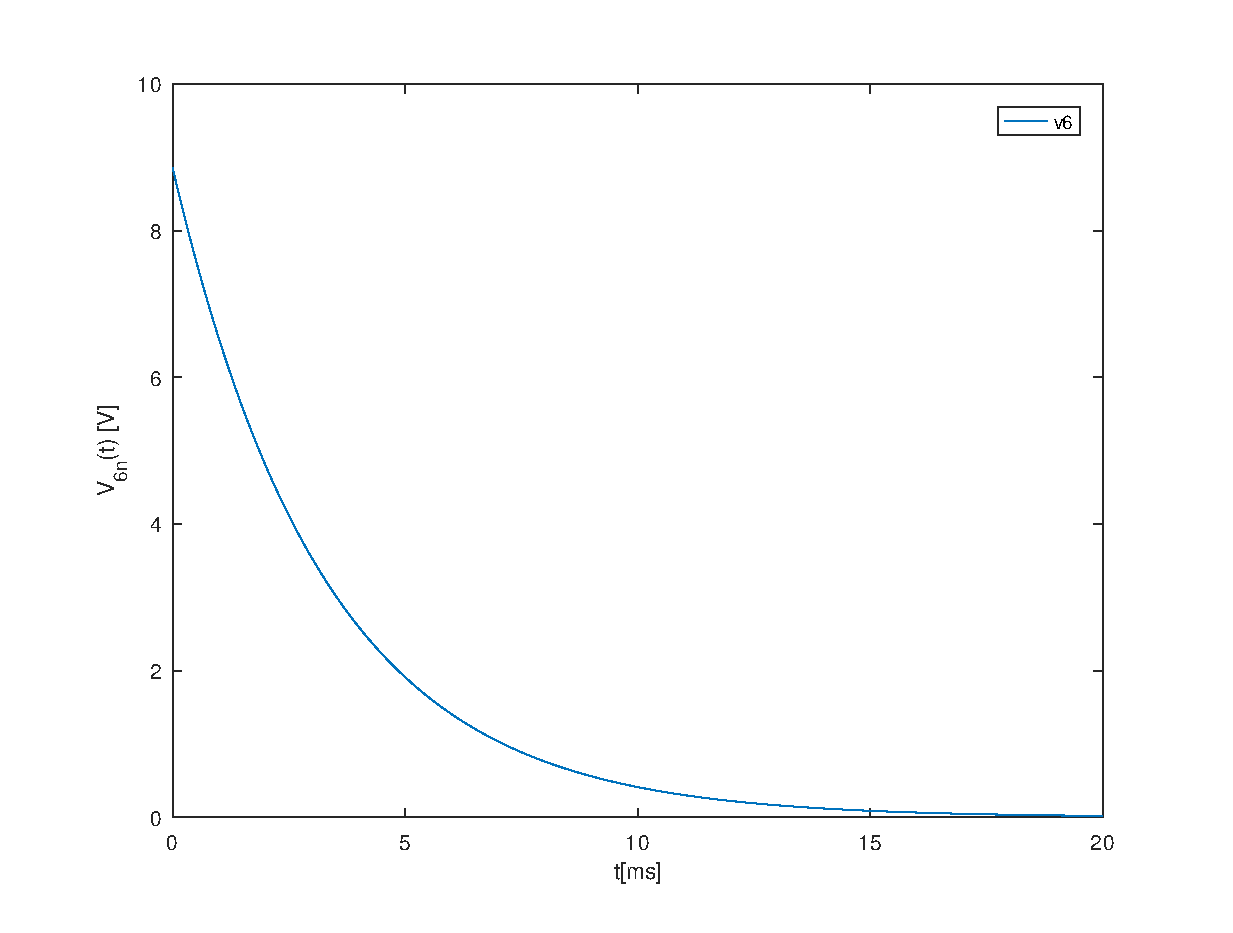
\includegraphics[width=0.8\linewidth]{theoretical_3.eps}
\label{fig:theoretical_3}
\end{figure}


%---------------Theoretical Analysis Exercise 4--------------------------------------------------------%
\subsection{Exercise 4}
\label{sec:exercise4}


For this exercise, to find the forced solution $V_6f$(t), we will work with the frequency f = 1000 Hz and the phasor voltage source $V_s$. Since the voltage source for t>0 is $v_s$(t) = sen(2$\pi$ft), to simplify the calculations and as suggested, we will work with the absolute of $V_s$, which was given and it is 1V. 

The node analysis for this exercise is pretty similar to the one in \ref{sec:exercise1} as the voltage source is once again $V_s$ and the capacitor no longer works as a voltage source. This means that we now have 7 varibles $V_1$, $V_2$, $V_3$, $V_5$, $V_6$, $V_7$ and $V_8$ and we can use the node method in nodes 2, 3, 6 and 7, since all the other ones are connected to voltage sources.

Equations \ref{node42} to \ref{supernode4} were all obtained from the node analysis in exercise 1. The first three are achieved, correspondingly, by nodes 2,3 and 7. The second to last equation refers to the current controlled voltage source $V_d$. Finally, the last one is the supernode that we got from merging the two branches placed on the left side of circuit.

\begin{equation}
  (V_{3} - V_{1})G_{1} + (V_{2} - V_{3})G_{2} + (V_{2} - V_{5})G_{3}= 0,
  \label{eq:node42}
\end{equation}

\begin{equation}
  (V_{3} - V_{2})G_{2} - (V_{2} - V_{5})K_{b} = 0,
  \label{eq:node43}
\end{equation}


\begin{equation}
  V_{7}G_{6} + (V_{7} - V_{8})G_{7} = 0,
  \label{eq:node47}
\end{equation}


\begin{equation}
  -V_{7}G_{6}K_{d} - (V_{5} - V_{8}) = 0,
  \label{eq:vd4}
\end{equation}

\begin{equation}
  (V_{1} - V_{2})G_{1} - V_{5}G_{7} - V_{7}G_{6} = 0,
  \label{eq:supernode4}
\end{equation}

The seventh and final equation (\ref{eq:node67}) necessary to complete the matrix is obtained by analysing node 6, using Kirchoff's Circuit Law and Ohm's Law for the resistor $R_5$. The equation for $V_b$ was secured previously (\ref{eq:vb1}). Because we are working with phasors, equations \ref{eq:caphasor1} and \ref{eq:caphasor2} are used to figure out the current flowing through the capacitor, by using its impendance $Z_c$.

\begin{equation}
  I_{c}Z_{c} = V_{c},
  \label{eq:caphasor1}
\end{equation}

\begin{equation}
  Z_{c} = \frac{1}{jwC},
  \label{eq:impedancecap}
\end{equation}

\begin{equation}
 Y_{c} = \frac{1}{Z_c},
  \label{eq:caphasor2}
\end{equation}

\begin{equation}
   (V_{6} - V_{5})G_{5} + (V_{2} - V_{5})K_{b} + (V_{6} - V_{8})Y_{c} = 0,
  \label{eq:node67}
\end{equation}

From this we get the following matrix. Knowing that $w = 2\pi*f$ with $f = 1kHz$, the matricial equation was solved in Octave. The results are printed on the table~\ref{table:??}.

\begin{equation}
\left[ \begin{array}{ccccccc} 
		1 & 0 & 0 & 0 & 0 & 0 & 0 \\ 
		-G_1 & G_1+G_2+G_3 & -G_2 & -G_3 & 0 & 0 & 0 \\
		0 & -G_2-K_b & G_2 & K_b & 0 & 0 & 0 \\ 
		0 & K_b & 0 & -K_b-G_5 & G_5+Y_c & 0 & -Y_c  \\ 
		0 & 0 & 0 & 0 & 0 & G_6+G_7 & -G_7  \\ 
		G_1 & -G_1 & 0 & -G_4 & 0 & -G_6 & 0  \\ 
		0 & 0 & 0 & -1 & 0 & -K_dG_6 & 1 \\ 

\end{array} \right]
\times \left[ \begin{array}{c} V_1 \\ V_2 \\ V_3 \\  V_5 \\ V_6 \\ V_7 \\ V_8 \end{array} \right] =
\left[ \begin{array}{c} V_s \\ 0 \\ 0 \\ 0 \\ 0 \\ 0 \\ 0  \end{array} \right]
\label{eq:nodalmatrix4}
\end{equation}

\begin{table}[!ht]
\centering
\begin{tabular}{ |c|c| }
\hline
 {\bf Node} & {\bf Complex amplitude} \\ 
 \hline\hline
 $V_{1}$ & $(\partialinput{1}{1}{theoretical_4.tex})*exp(j*\partialinput{8}{8}{theoretical_4.tex})$   \\
 \hline
 $V_{2}$ & $(\partialinput{2}{2}{theoretical_4.tex})*exp(j*\partialinput{9}{9}{theoretical_4.tex})$   \\
 \hline
 $V_{3}$ & $(\partialinput{3}{3}{theoretical_4.tex})*exp(j*\partialinput{10}{10}{theoretical_4.tex})$   \\
 \hline
 $V_{5}$ & $(\partialinput{4}{4}{theoretical_4.tex})*exp(j*\partialinput{11}{11}{theoretical_4.tex})$   \\
 \hline
 $V_{6}$ & $(\partialinput{5}{5}{theoretical_4.tex})*exp(j*\partialinput{12}{12}{theoretical_4.tex})$   \\
 \hline
 $V_{7}$ & $(\partialinput{6}{6}{theoretical_4.tex})*exp(j*\partialinput{13}{13}{theoretical_4.tex})$   \\
 \hline
 $V_{8}$ & $(\partialinput{7}{7}{theoretical_4.tex})*exp(j*\partialinput{14}{14}{theoretical_4.tex})$   \\
 \hline
\end{tabular}
\caption{Complex amplitudes in all nodes(Exercise 4)}
\label{table:theoretical_4}
\end{table}

\begin{figure}[!ht] \centering
\caption{Forced solution $v_{6f}(t)$ for $f=1KHz$ in the interval $[-5,20]ms$}
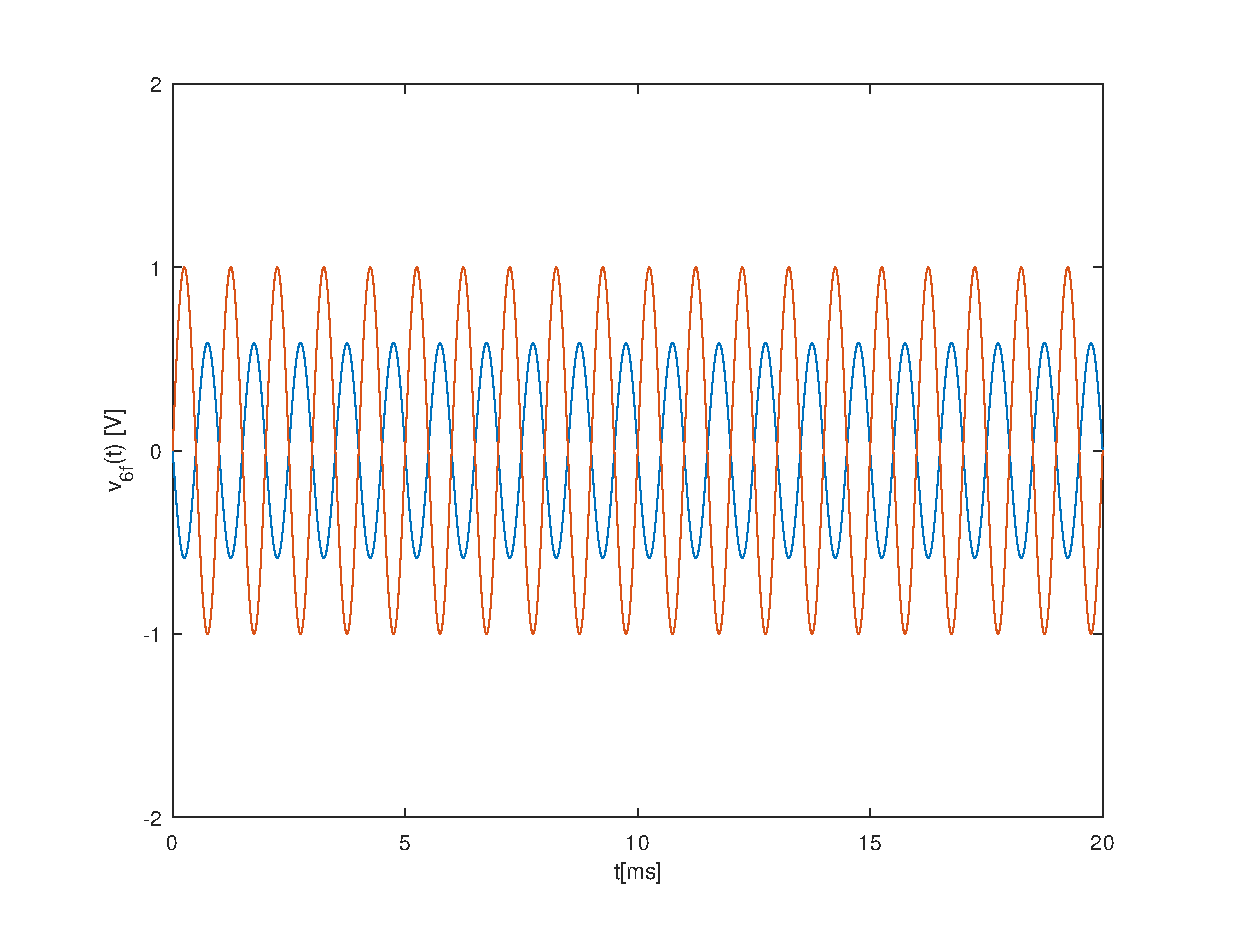
\includegraphics[width=0.8\linewidth]{theoretical_4.eps}
\label{fig:theoretical_4}
\end{figure}

%---------------Theoretical Analysis Exercise 5--------------------------------------------------------%
\newpage
\subsection{Exercise 5}
\label{sec:exercise5}

%%%%%%%%%%%%%%%%%% NAO SEI A EXPRESSAO DE V6 FORÇADO
%%%%%%%%%%%%%%%%%%%%%%%%%%%%%%%%%%%%%%%%%%%%%%%%%

To figure out $V_6$, we simply had to convert the phasor to real time fuctions, being so that the value of $V_6$ is just the sum of the natural solution with the forced solution, calculated in exercises 3 and 4. The equation for $V_s$(t) is given and it is written below, as the one for $V_6$(t). The frequency used was 1000 Hz. 

\begin{equation}
   V_{s}(t) =  \sin{2{\pi}ft},
  \label{eq:vsgiven}
\end{equation}

\begin{equation}
  V_{6}(t) = (V_{x} + V_{8})e^{-\frac{t}{RC}} + V_{6f}(t),
  \label{eq:v6tot}
\end{equation}

Finally, in figure \ref{fig:theoretical_5}, we have the graph for both $V_s$ and $V_6$ in function of t, in the interval [-5, 20] ms. As stated in the simultation analyis, it was expected for $V_s$ to not show a frequency response, since it is the source of frequency change. The same is not the case for $V_6$ as is depends on $V_s$.

\begin{figure}[!ht] \centering
\caption{Final solution of $v_6(t)$ and $v_s(t)$ in the interval $[-5,20]ms$}
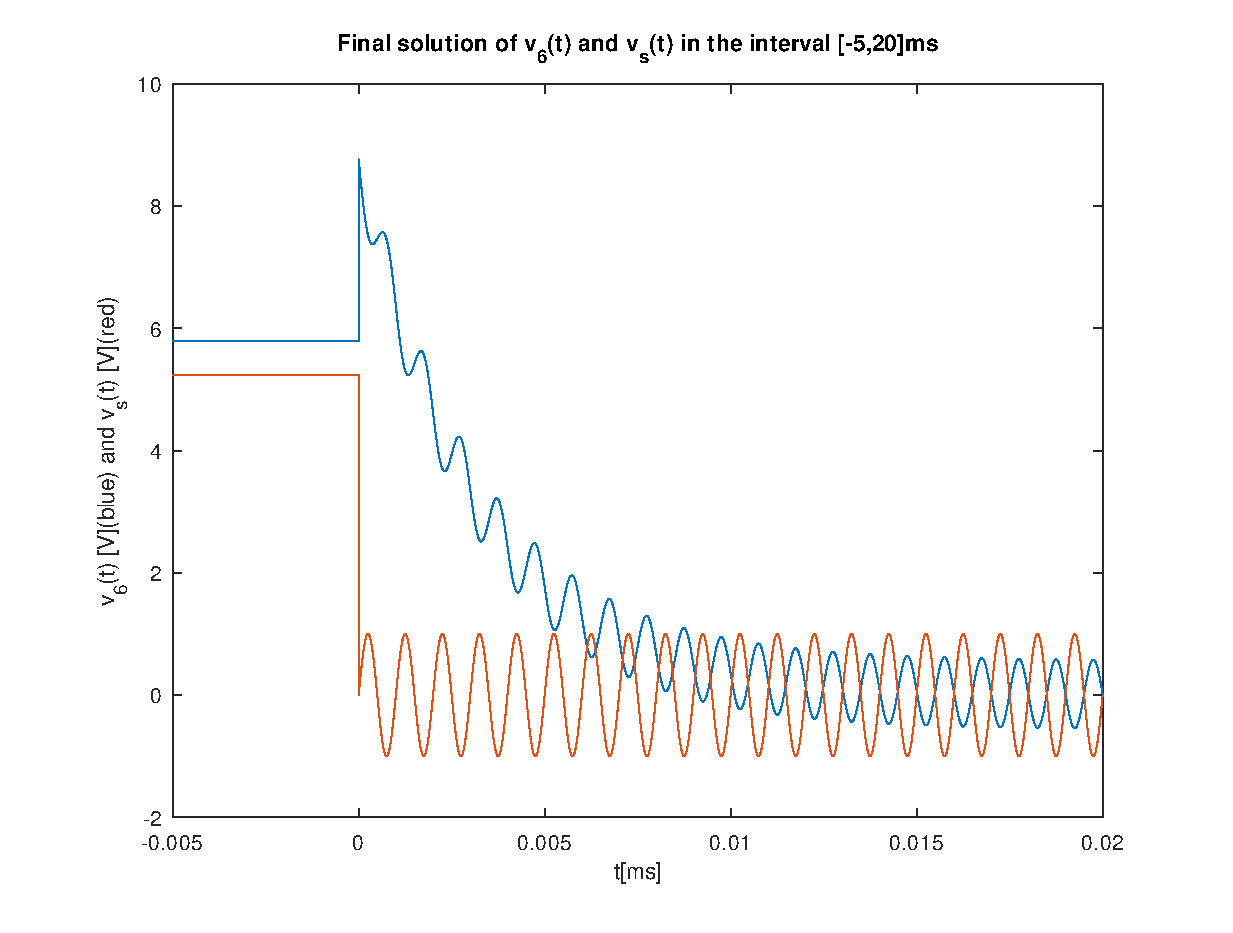
\includegraphics[width=0.8\linewidth]{theoretical_5.eps}
\label{fig:theoretical_5}
\end{figure}

%---------------Theoretical Analysis Exercise 6--------------------------------------------------------%
\newpage
\subsection{Exercise 6}
\label{sec:exercise6}


\begin{figure}[!ht] 
\caption{Frequency response, $v_{c}(f)$, $v_6(f)$, and $v_s(f)$ in $V$. Magnitude in $dB$ and Phase is in degrees}
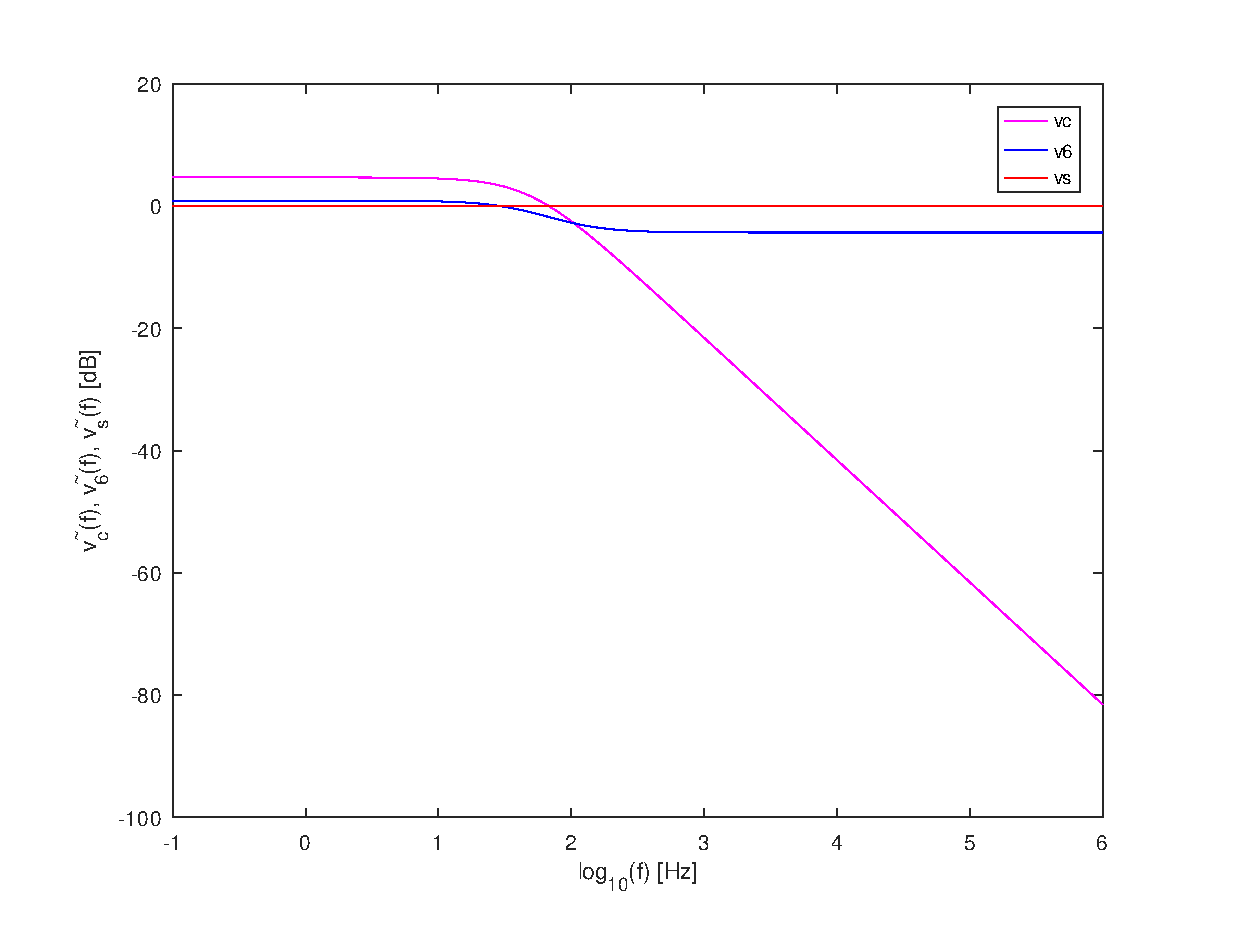
\includegraphics[width=0.55\textwidth]{theoretical_6_dB.eps}
\hfill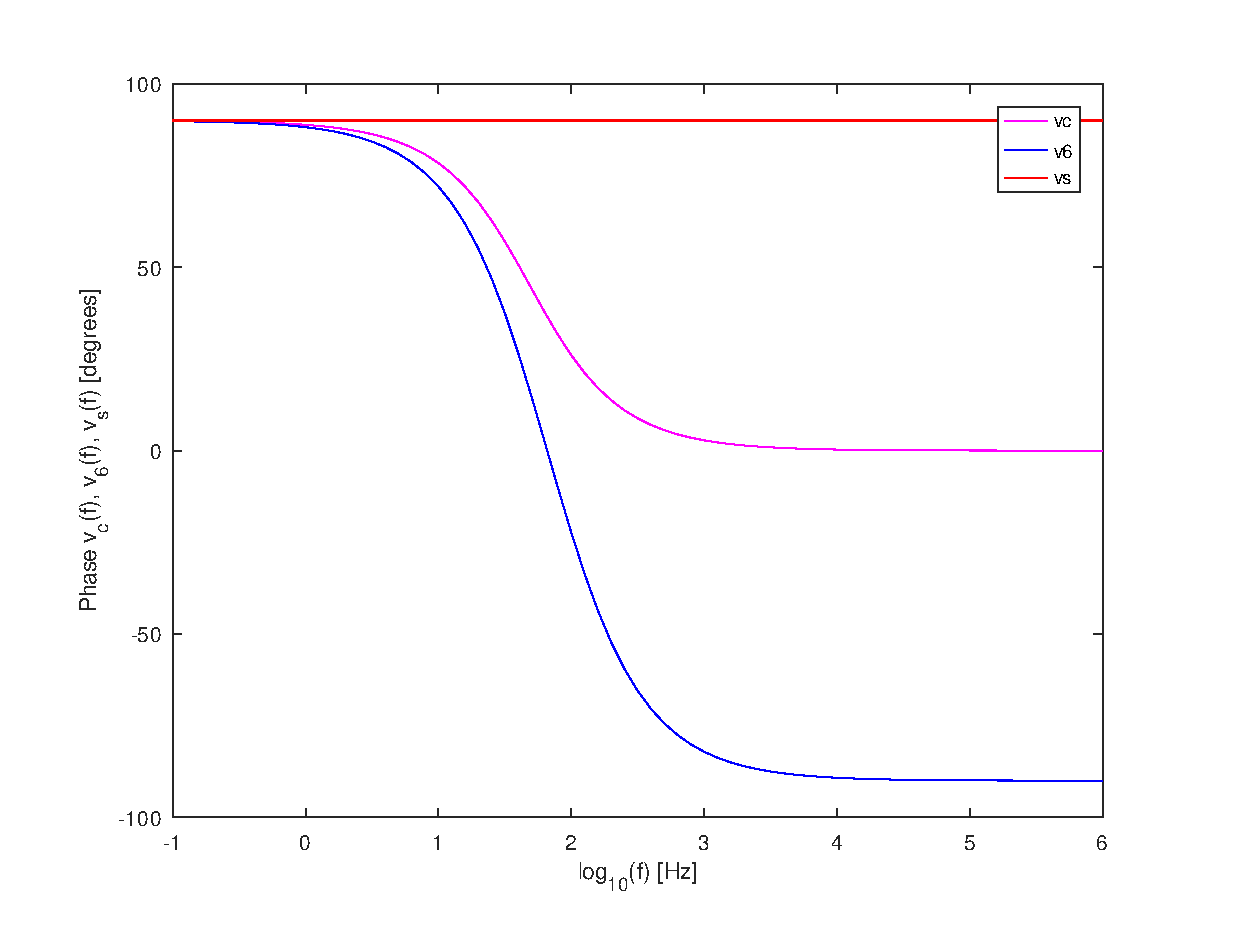
\includegraphics[width=0.55\textwidth]{theoretical_6_phase.eps}
\label{fig:theoretical_6}
\end{figure}








\newpage
\section{Simulation Analysis}
\label{sec:simulation}


\subsection{Exercise 1}
\label{Exercise 1}

%---------------Simulation Analysis Exercise 1--------------------------------------------------------%
In this section we proceed to do the anlysis of the circuit through the use of the Ngspice simulation programm. In figure~\ref{fig:circuit_simulation} we have the circuit that was inputed into Ngspice (and also the considered current flows and nodes). The file can be found at the $sim$ folder inside the $T2$ folder.

\begin{figure}[!ht] \centering
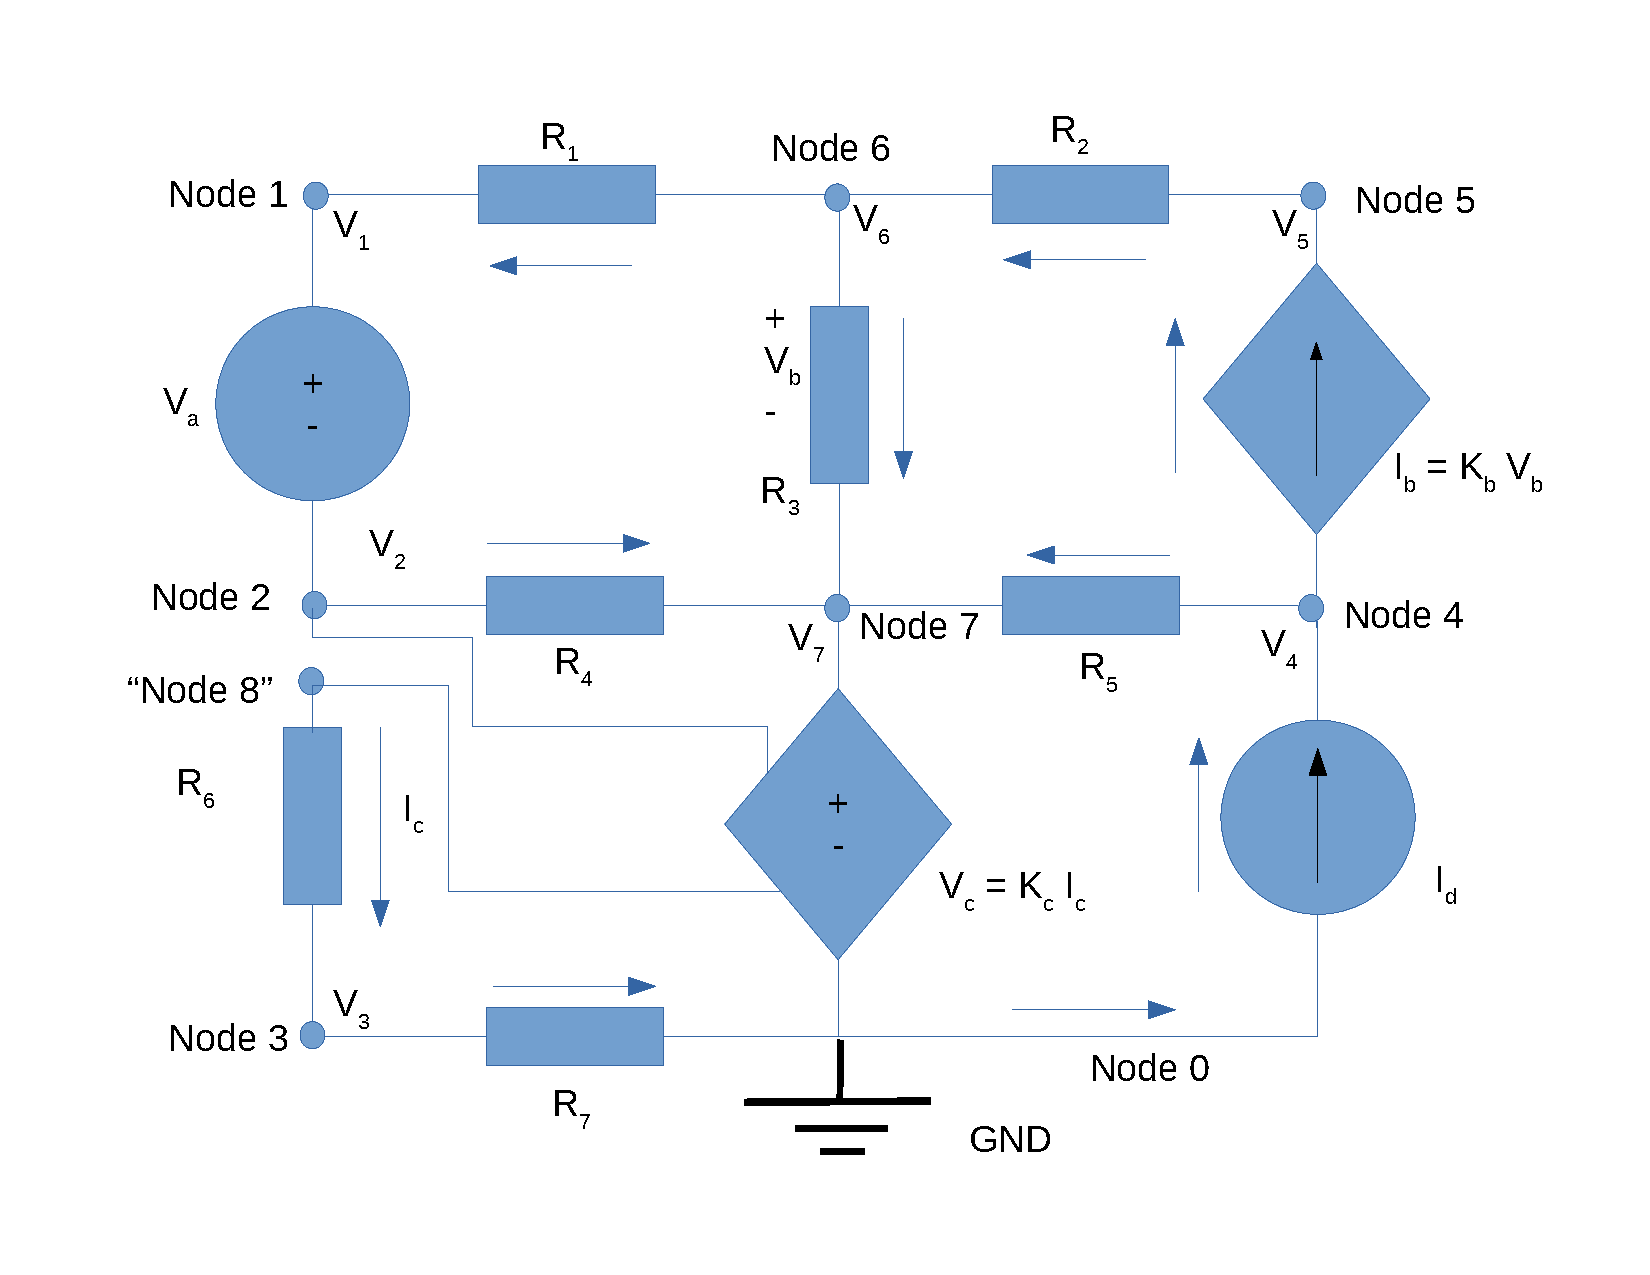
\includegraphics[width=0.8\linewidth]{circuit_simulation.pdf}
\caption{Considered circuit for Ngspice simulation}
\label{fig:circuit_simulation}
\end{figure}

$V_9$ refers to an extra ficticious node created specifically for the Ngspice simulation, and it is below $0(GND)$ and above resistor R6 as it can be seen above in figure~\ref{fig:circuit_simulation}.The reason this node is necessary is because when creating a current controlled voltage source, Ngspice gets the current value by refering to a voltage source from where the current goes through. Since $I_d$ does not go through any voltage source in the circuit (does not go through $V_s$) we used this extra node to create a voltage source of 0$V$ (Which can be confirmed since $V_9 = $GND$ = 0$) from which we are certain $I_d$ is passing by. 

Table~\ref{tab:op} shows the simulated operating point results for the circuit
under analysis given the values found on Table~\ref{tab:op}. The variables representation and format are automatically determined by Ngspice.

\begin{table}[!ht]
  \centering
  \begin{tabular}{|l|r|}
    \hline    
    {\bf Name} & {\bf Value [A or V]} \\ \hline
    @c1[i] & 0.000000e+00\\ \hline
@gib[i] & -2.45467e-04\\ \hline
@r1[i] & 2.344922e-04\\ \hline
@r2[i] & 2.454667e-04\\ \hline
@r3[i] & 1.097445e-05\\ \hline
@r4[i] & 1.220071e-03\\ \hline
@r5[i] & 2.454667e-04\\ \hline
@r6[i] & 9.855785e-04\\ \hline
@r7[i] & 9.855785e-04\\ \hline
v1 & 5.242048e+00\\ \hline
v2 & 5.002985e+00\\ \hline
v3 & 4.499645e+00\\ \hline
v5 & 5.036927e+00\\ \hline
v6 & 5.789615e+00\\ \hline
v7 & -1.98352e+00\\ \hline
v8 & -2.97405e+00\\ \hline
v9 & 0.000000e+00\\ \hline

  \end{tabular}
  \caption{Operating point. A variable preceded by @ is of type {\em current}
    and expressed in Ampere; other variables are of type {\it voltage} and expressed in
    Volt. (the g in "gib" refers to the Ngspice notation of a voltage controlled current source)}
  \label{tab:op}
\end{table}

We can get all the missing values given the equations showed in section~\ref{sec:analysis}.

\begin{equation}
  V_c = V_7
  \label{eq:1}
\end{equation}

\begin{equation}
  V_b = V_6 - V_7
  => V_b = -3.3943*10^{-2} V
\end{equation}

From Table~\ref{tab:op} we can directly get the value of $I_d$:

\begin{equation}
  I_d = @r6[i]
\end{equation}

With this we have finalized the circuit anlysis through simulation with Ngspice.














\newpage
\section{Conclusion}
\label{sec:conclusion}

In this laboratory we dimensioned and implemented a BandPass Filter (BPF) using an OP-AMP.

We can now compare the obtained results by theory and by simulation:

\begin{table}[h]
    \centering
    \begin{tabular}{|c|c|c|}
    \hline
    {\bf Parameter} & {\bf Theoretical Value}& {\bf Simulation Value}\\
    \hline\hline
     Low Frequency [Hz] & 415.55 & 418.14\\
    \hline
    High Frequency [Hz] & 2531.6 & 2352.9\\
    \hline
   Central Frequency [Hz] & 1025.7 & 991.9\\
   \hline
     $Z{input}$ & 1154.7 & 1154.8 \\
    \hline
     $Z{output}$ & 720.25 & 724.01\\
    \hline
      Gain [db] & 40.037 & 39.949\\
    \hline
    \end{tabular}
    \caption{Comparison of the theoretical and simulation values.}
    \label{tab:values}
\end{table}

Contrary to our goal for the laboratory, there are some clear differences between the results. This could be due to the model applied in Ngspice being much more realistic as well as its parameters being more complex than the one analysed in the theoretical part or the fact that the components of the circuit, specially the OP-AMP, are not linear. 
Despite all of this, we are satisfied with our results and we consider the model used to be valid.


Final merit obtained was 8.4318e-06 (Ngspice)

Below are the two plots for comparison:

\begin{figure}[!ht] \centering
\caption{Frequency response $V_o$(f)/$V_i$(f)}
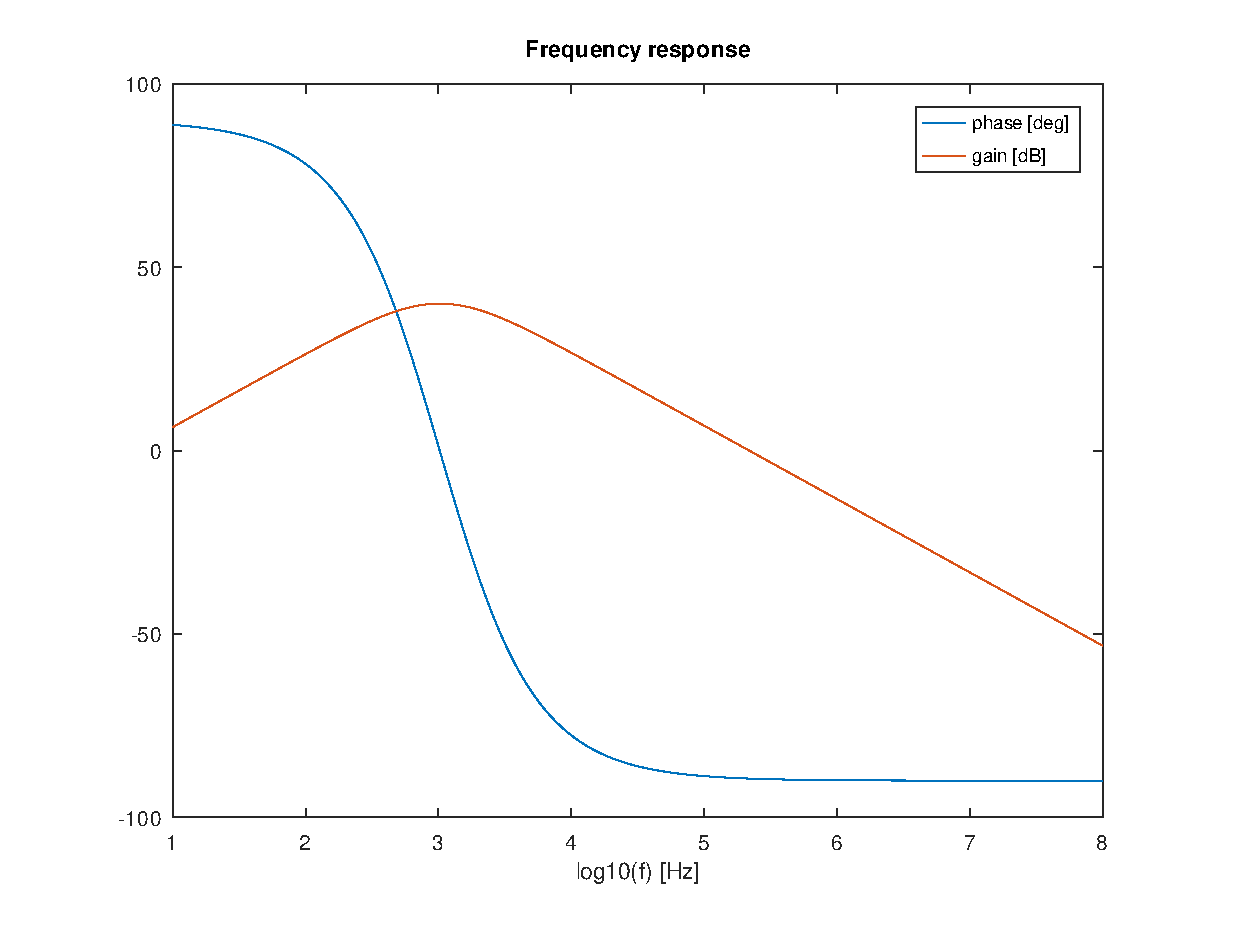
\includegraphics[width=0.4\linewidth]{theory.eps}
\caption{Frequency response for the simulation analysis}
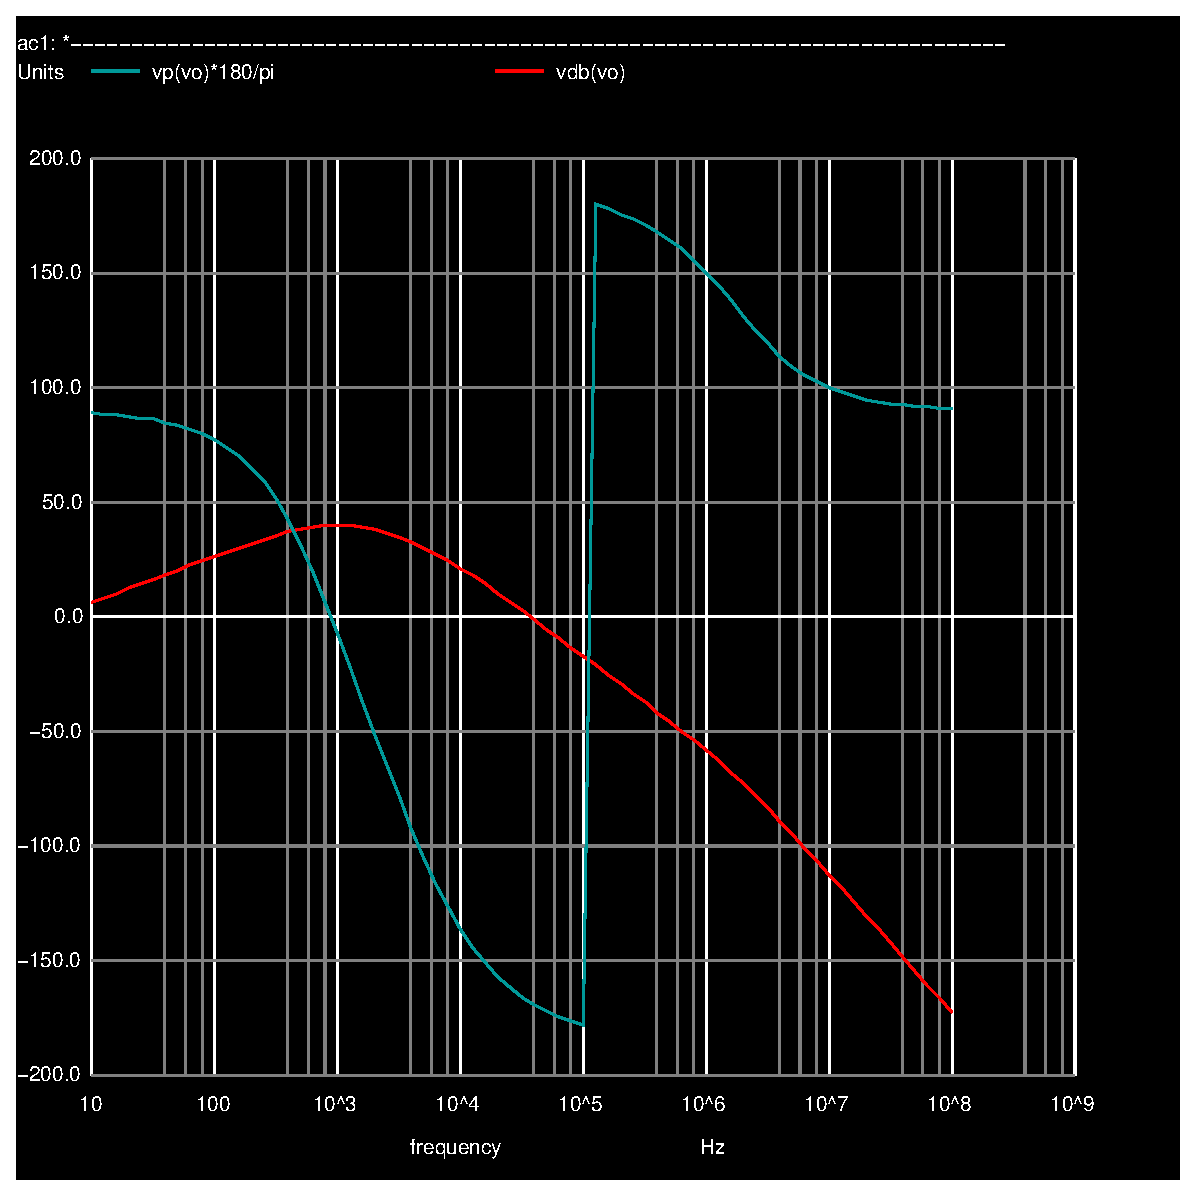
\includegraphics[width=0.4\linewidth]{simulation.eps}
\label{fig:theoretical}
\end{figure}


%\cleardoublepage

% ----------------------------------------------------------------------
%  Bibliography
% ----------------------------------------------------------------------
%\addcontentsline{toc}{section}{\bibname}
%\bibliographystyle{abbrvunsrtnat} % <<<<< SELECT IF USING REFERENCES BY NUMBER (CITATION ORDER)
%\bibliography{../../../BIBfile.bib}

% ----------------------------------------------------------------------
\end{document}
% ----------------------------------------------------------------------

